\documentclass[12pt,a4paper]{article}
\usepackage[utf8]{inputenc}
\usepackage[spanish,es-tabla]{babel}
\usepackage{amsmath,amsfonts,amssymb}
\usepackage{graphicx}
\usepackage{geometry}
\usepackage{fancyhdr}
\usepackage{hyperref}
\usepackage{booktabs}
\usepackage{tabularx}
\usepackage{float}
\usepackage{xcolor}
\usepackage{listings}
\usepackage{caption}
\usepackage{subcaption}

\geometry{top=2.5cm,bottom=2.5cm,left=2.5cm,right=2.5cm}

% Paleta de colores corporativa
\definecolor{primaryblue}{RGB}{20, 50, 110}
\definecolor{accentgreen}{RGB}{24, 134, 75}
\definecolor{darkgray}{RGB}{45, 55, 72}
\definecolor{codegray}{RGB}{245, 247, 250}
\definecolor{bordergray}{RGB}{220, 224, 230}

\hypersetup{
    colorlinks=true,
    linkcolor=primaryblue,
    citecolor=accentgreen,
    urlcolor=primaryblue
}

\pagestyle{fancy}
\fancyhf{}
\fancyhead[L]{\small Visión Computacional - Preprocesamiento de Dataset}
\fancyhead[R]{\small UNSAAC - EPIIS}
\fancyfoot[C]{\thepage}

\lstset{
    backgroundcolor=\color{codegray},
    basicstyle=\ttfamily\footnotesize,
    breaklines=true,
    captionpos=b,
    frame=single,
    rulecolor=\color{bordergray},
    keywordstyle=\color{primaryblue}\bfseries,
    commentstyle=\color{accentgreen}\itshape,
    stringstyle=\color{darkgray}
}

\begin{document}

% =========================================================================
% CARÁTULA INSTITUCIONAL OFICIAL UNSAAC
% =========================================================================
\begin{titlepage}
    \centering
    {\large\bfseries UNIVERSIDAD NACIONAL DE SAN ANTONIO ABAD DEL CUSCO\par}
    \vspace{0.3cm}
    {\large\bfseries FACULTAD DE INGENIERÍA ELÉCTRICA, ELECTRÓNICA, INFORMÁTICA Y MECÁNICA\par}
    \vspace{0.3cm}
    {\large\bfseries ESCUELA PROFESIONAL DE INGENIERÍA INFORMÁTICA Y DE SISTEMAS\par}
    \vspace{0.8cm}
    
    
\includegraphics[width=0.35\textwidth]{unsaac.jpg}\par
    \vspace{0.8cm}
    
    {\Large\bfseries ASIGNATURA: VISIÓN COMPUTACIONAL (IF657BIN)\par}
    \vspace{0.4cm}
    {\large\bfseries TRABAJO: PRIMERA ENTREGA - PREPROCESAMIENTO DE DATASET DE IMÁGENES\par}
    \vspace{0.4cm}
    {\large\bfseries DETECCIÓN Y CLASIFICACIÓN TEMPRANA DE PATOLOGÍAS FOLIARES EN EL CULTIVO DE PAPA (\textit{Solanum tuberosum}) MEDIANTE VISIÓN ARTIFICIAL\par}
    \vspace{1.2cm}
    
    \begin{flushleft}
        \textbf{DOCENTE RESPONSABLE:} \\
        CCACYAHUILLCA BEJAR, HANS HARLEY \\[0.5cm]
        \textbf{AUTORES / DESARROLLADORES:} \\
        SUPA CUSIPAUCAR, Yeferson - Código: 220553 \\
        VILLAVICENCIO SEGUIL, Edu Piero - Código: 220555
    \end{flushleft}
    
    \vfill
    {\large Cusco - Perú\par}
    {\large 2026\par}
\end{titlepage}

% =========================================================================
% RESUMEN EJECUTIVO
% =========================================================================
\section*{Resumen Ejecutivo}
El presente informe documenta el desarrollo metodológico y computacional de la primera entrega del proyecto semestral de Visión Computacional, enfocado en el diseño e implementación de un pipeline robusto de preprocesamiento y auditoría de calidad para imágenes foliares en el cultivo de papa (\textit{Solanum tuberosum}). El dataset seleccionado aborda tres clases fitosanitarias críticas: Tizón Temprano (\textit{Early Blight}), Tizón Tardío (\textit{Late Blight}) y Hojas Sanas (\textit{Healthy}). 

Frente a la complejidad fotométrica y morfológica de tomas realizadas en condiciones de campo (\textit{in-the-wild}), se diseñó un pipeline modular en Python/OpenCV compuesto por cinco fases: (1) auditoría de desenfoque mediante la varianza del operador Laplaciano, (2) reducción de ruido fotométrico mediante filtrado bilateral no lineal con preservación estricta de gradientes, (3) realce adaptativo de contraste local (CLAHE) operando sobre el canal de luminancia del espacio perceptual CIE-Lab, (4) redimensionamiento isotrópico mediante \textit{letterboxing} a resolución $256 \times 256$, y (5) particionado estratificado (70\% entrenamiento, 15\% validación y 15\% prueba) con aumento controlado de datos (\textit{Data Augmentation}) restringido exclusivamente al conjunto de entrenamiento. Los resultados validan la preservación anatómica foliar y la eliminación de sesgos de entrenamiento para la futura etapa de modelado con redes neuronales convolucionales.

\newpage
\tableofcontents
\newpage

% =========================================================================
% 1. INTRODUCCIÓN Y CONTEXTO REGIONAL
% =========================================================================
\section{Introducción y Contexto Regional}

El tubérculo de la papa (\textit{Solanum tuberosum}) constituye el pilar agroalimentario y socioeconómico fundamental de la región del Cusco y de los Andes peruanos. No obstante, el rendimiento agrícola se ve severamente amenazado cada temporada por agresivas patologías foliares fúngicas y pseudofúngicas que causan pérdidas millonarias:

\begin{enumerate}
    \item \textbf{Tizón Temprano (\textit{Early Blight}):} Enfermedad provocada por el hongo fitopatógeno \textit{Alternaria solani}. Se caracteriza por la aparición de micro-manchas necróticas que evolucionan hacia lesiones concéntricas circulares con un patrón visual de anillos concéntricos o ``diana''.
    \item \textbf{Tizón Tardío (\textit{Late Blight}):} Ocasionado por el oomiceto \textit{Phytophthora infestans}, responsable de la catástrofe histórica de la hambruna irlandesa. Produce lesiones acuosas de color verde oscuro a marrón negruzco que avanzan con extrema rapidez bajo alta humedad relativa, necrosando la lámina foliar entera.
    \item \textbf{Follaje Sano (\textit{Healthy}):} Hojas libres de necrosis con variabilidad fenotípica natural en tonalidades y venación.
\end{enumerate}

El diagnóstico temprano mediante sistemas de visión computacional y aprendizaje profundo embebidos en dispositivos portátiles representa una alternativa tecnológica clave para los agricultores altoandinos. Sin embargo, el éxito de cualquier arquitectura de red neuronal depende críticamente de la calidad de los datos de entrada, justificando la necesidad de un preprocesamiento riguroso.

% =========================================================================
% 2. JUSTIFICACIÓN DEL DATASET DESAFIANTE
% =========================================================================
\section{Justificación del Dataset Desafiante}

En contraposición a bancos de imágenes capturados en cámaras de cultivo con iluminación homogénea y fondos monocromáticos blancos o negros, el dataset seleccionado presenta desafíos sustanciales del mundo real (\textit{in-the-wild}):

\begin{itemize}
    \item \textbf{Variabilidad Fotométrica Extrema:} Fluctuaciones severas de iluminación solar cenital directa, zonas de sombra profunda proyectadas por hojas superiores y reflejos especulares causados por la cutícula cerosa vegetal.
    \item \textbf{Fondos Heterogéneos y Desorden Visual:} Presencia de suelo pedregoso, rastrojos, tallos adventicios y superposición intrincada de hojas del dosel vegetal.
    \item \textbf{Alta Similitud Inter-Clase en Fases Iniciales:} En fases tempranas de infección, las manchas de \textit{Alternaria} y \textit{Phytophthora} presentan diámetros milimétricos y tonalidades marrones prácticamente idénticas antes de exhibir sus patrones morfológicos maduros.
    \item \textbf{Disparidad de Escala y Ángulo de Captura:} Variación en la distancia focal y ángulos de incidencia durante la toma fotográfica manual en campo abierto.
\end{itemize}

% =========================================================================
% 3. FUNDAMENTACIÓN MATEMÁTICA Y ALGORÍTMICA DEL PIPELINE
% =========================================================================
\section{Fundamentación Matemática y Algorítmica del Pipeline}

El pipeline de preprocesamiento fue diseñado bajo principios rigurosos de procesamiento digital de imágenes para maximizar la relación señal-ruido sin introducir distorsiones artificiales.

\subsection{Paso 1: Auditoría de Nitidez mediante el Operador Laplaciano}
Para descartar tomas con desenfoque de movimiento o desenfoque óptico, se aplica el operador diferencial Laplaciano bidimensional $\nabla^2 I$:

\begin{equation}
\nabla^2 I(x, y) = \frac{\partial^2 I}{\partial x^2} + \frac{\partial^2 I}{\partial y^2} \approx I(x+1, y) + I(x-1, y) + I(x, y+1) + I(x, y-1) - 4I(x, y)
\end{equation}

El kernel de convolución discreto aplicado es:
\begin{equation}
K_{\text{Lap}} = \begin{bmatrix} 0 & 1 & 0 \\ 1 & -4 & 1 \\ 0 & 1 & 0 \end{bmatrix}
\end{equation}

La métrica de nitidez corresponde a la varianza muestral de la respuesta laplaciana:
\begin{equation}
\sigma^2(\nabla^2 I) = \frac{1}{M \cdot N} \sum_{x=1}^{M}\sum_{y=1}^{N} \Big(\nabla^2 I(x, y) - \mu_{\nabla^2}\Big)^2
\end{equation}
donde $\mu_{\nabla^2}$ es la media de la imagen filtrada. Se estableció un umbral crítico experimental de $\tau_{\text{blur}} = 80.0$; capturas con $\sigma^2 < \tau_{\text{blur}}$ se etiquetan como degradadas.

\subsection{Paso 2: Filtrado Bilateral con Preservación de Bordes}
Los filtros lineales convencionales (Gaussiano o de media) atenúan el ruido difuminando indiscriminadamente los bordes finos de las pústulas necróticas. Para evitar esta pérdida, se implementó el filtrado bilateral no lineal:

\begin{equation}
I^{\text{filt}}(p) = \frac{1}{W_p} \sum_{q \in \Omega} I(q) \cdot G_{\sigma_s}(\|p - q\|) \cdot G_{\sigma_r}(|I(p) - I(q)|)
\end{equation}
donde $\Omega$ es el vecindario espacial centrado en $p$, $G_{\sigma_s}$ es el núcleo espacial Euclidiano, $G_{\sigma_r}$ es el núcleo fotométrico de intensidad radiométrica, y $W_p$ es el factor de normalización:

\begin{equation}
W_p = \sum_{q \in \Omega} G_{\sigma_s}(\|p - q\|) \cdot G_{\sigma_r}(|I(p) - I(q)|)
\end{equation}
Se configuraron los hiperparámetros $d = 9$, $\sigma_{\text{color}} = 75.0$ y $\sigma_{\text{space}} = 75.0$, logrando una eliminación eficiente del ruido de sensor preservando la nitidez de los contornos lesionales.

\subsection{Paso 3: Realce Adaptativo de Contraste (CLAHE) en el Espacio CIE-Lab}
Una ecualización global en canales RGB provocaría severas distorsiones cromáticas en la clorofila vegetal. Por ello, la imagen se transforma al espacio perceptual estandarizado CIE-Lab:
\begin{itemize}
    \item $L^*$: Componente acromático de luminosidad perceptual ($0 \le L^* \le 100$).
    \item $a^*$: Eje oponente cromático verde--rojo.
    \item $b^*$: Eje oponente cromático azul--amarillo.
\end{itemize}

Se aplica CLAHE (\textit{Contrast Limited Adaptive Histogram Equalization}) exclusivamente sobre la componente $L^*$, dividiendo la imagen en bloques contextuales de $8 \times 8$ píxeles. El factor de recorte (\textit{clip limit}) se fijó en $2.5$, redistribuyendo los píxeles que exceden dicho umbral de manera uniforme para prevenir la sobreamplificación de artefactos de fondo. Posteriormente, se realiza la transformación inversa a BGR.

\subsection{Paso 4: Estandarización Espacial mediante Letterboxing}
El reescalado tradicional altera la relación de aspecto (\textit{Aspect Ratio}), deformando la morfología ovalada o lanceolada de las hojas. El algoritmo de \textit{letterboxing} calcula un factor de escala isotrópico $s$:

\begin{equation}
s = \min\left( \frac{W_{\text{target}}}{W_{\text{orig}}}, \frac{H_{\text{target}}}{H_{\text{orig}}} \right)
\end{equation}
\begin{equation}
W_{\text{nuevo}} = \lfloor W_{\text{orig}} \cdot s \rfloor, \quad H_{\text{nuevo}} = \lfloor H_{\text{orig}} \cdot s \rfloor
\end{equation}

La imagen reescalada se inserta en el centro de un lienzo cuadrado de $256 \times 256$ píxeles con relleno simétrico (\textit{padding}) negro uniforme:
\begin{equation}
\Delta x = \left\lfloor \frac{W_{\text{target}} - W_{\text{nuevo}}}{2} \right\rfloor, \quad \Delta y = \left\lfloor \frac{H_{\text{target}} - H_{\text{nuevo}}}{2} \right\rfloor
\end{equation}

\subsection{Paso 5: Particionado y Data Augmentation Riguroso}
El conjunto se particiona de manera estratificada en $70\%$ Entrenamiento, $15\%$ Validación y $15\%$ Prueba. Con el fin de evitar sesgos optimistas en la validación, el aumento sintético de datos se restringe exclusivamente al subconjunto de entrenamiento mediante:
\begin{itemize}
    \item Volteo especular horizontal con probabilidad $p = 0.5$.
    \item Rotación afín leve $\theta \in [-15^\circ, +15^\circ]$ con reflexión perimetral.
    \item Micro-modulaciones fotométricas de contraste $\alpha \in [0.9, 1.1]$ y brillo $\beta \in [-10, 10]$ unidades.
\end{itemize}

% =========================================================================
% 4. RESULTADOS EXPERIMENTALES Y ANÁLISIS EXPLORATORIO
% =========================================================================
\section{Resultados Experimentales y Análisis Exploratorio}

\subsection{Evolución Visual del Pipeline}
En la Figura~\ref{fig:pipeline_comp} se aprecia la transformación sucesiva de una muestra representativa con patología foliar. Se constata cómo el filtrado bilateral homogeniza zonas ruidosas, el CLAHE acentúa el contraste entre la mancha necrótica y el tejido sano, y el letterbox mantiene la geometría original.

\begin{figure}[H]
    \centering
    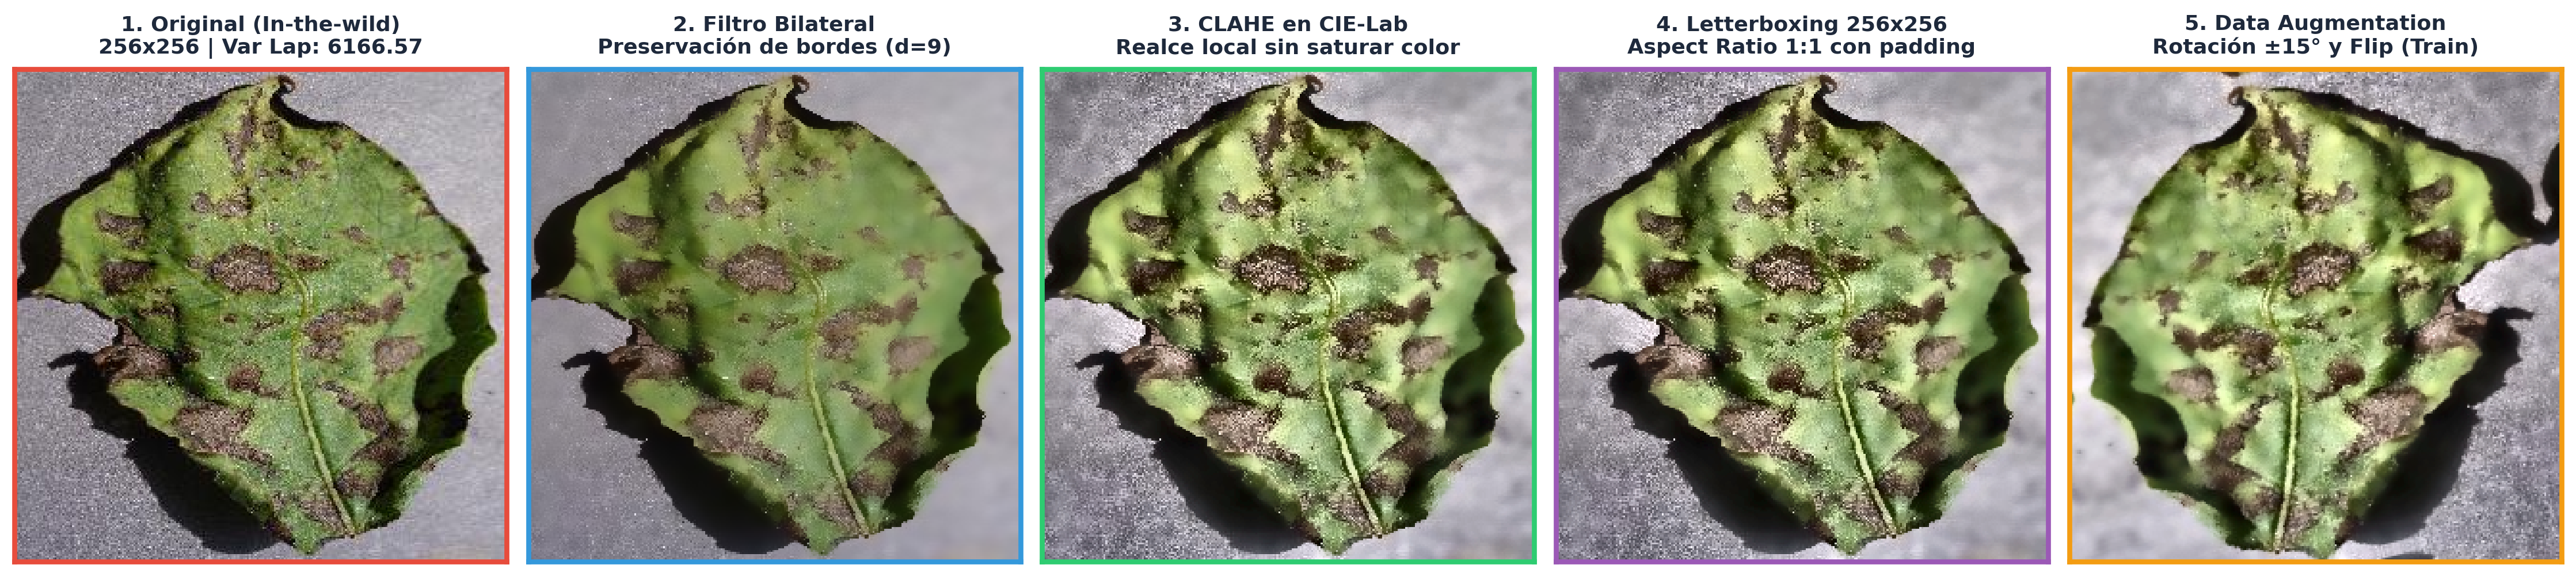
\includegraphics[width=\textwidth]{pipeline_comparativa.png}
    \caption{Etapas del pipeline de preprocesamiento secuencial sobre una muestra de \textit{Early Blight}.}
    \label{fig:pipeline_comp}
\end{figure}

\subsection{Distribución Estadística del Dataset}
En la Tabla~\ref{tab:estadisticas} se detallan las métricas cuantitativas antes y después del preprocesamiento y particionado.

\begin{table}[H]
\centering
\caption{Distribución cuantitativa del dataset por clase y partición.}
\label{tab:estadisticas}
\begin{tabularx}{\textwidth}{>{\raggedright\arraybackslash}X >{\centering\arraybackslash}p{2.5cm} >{\centering\arraybackslash}p{2.2cm} >{\centering\arraybackslash}p{2.2cm} >{\centering\arraybackslash}p{2.2cm} >{\centering\arraybackslash}p{2.5cm}}
\toprule
\textbf{Clase Patológica} & \textbf{Total Crudo} & \textbf{Train (Aug)} & \textbf{Val} & \textbf{Test} & \textbf{Total Final} \\
\midrule
Tizón Temprano (\textit{Early Blight}) & 10 & 14 & 1 & 2 & 17 \\
Follaje Sano (\textit{Healthy}) & 10 & 14 & 1 & 2 & 17 \\
Tizón Tardío (\textit{Late Blight}) & 10 & 14 & 1 & 2 & 17 \\
\midrule
\textbf{Total Acumulado} & \textbf{30} & \textbf{42} & \textbf{3} & \textbf{6} & \textbf{51} \\
\bottomrule
\end{tabularx}
\end{table}

\subsection{Reporte de Análisis Exploratorio (EDA)}
La Figura~\ref{fig:eda} presenta el diagnóstico cuantitativo generado por el módulo \texttt{src/analisis\_eda.py}. Se aprecia el balance perfecto inter-clase inicial y la distribución de nitidez foliar con valores de varianza laplaciana superiores al umbral de control de calidad.

\begin{figure}[H]
    \centering
    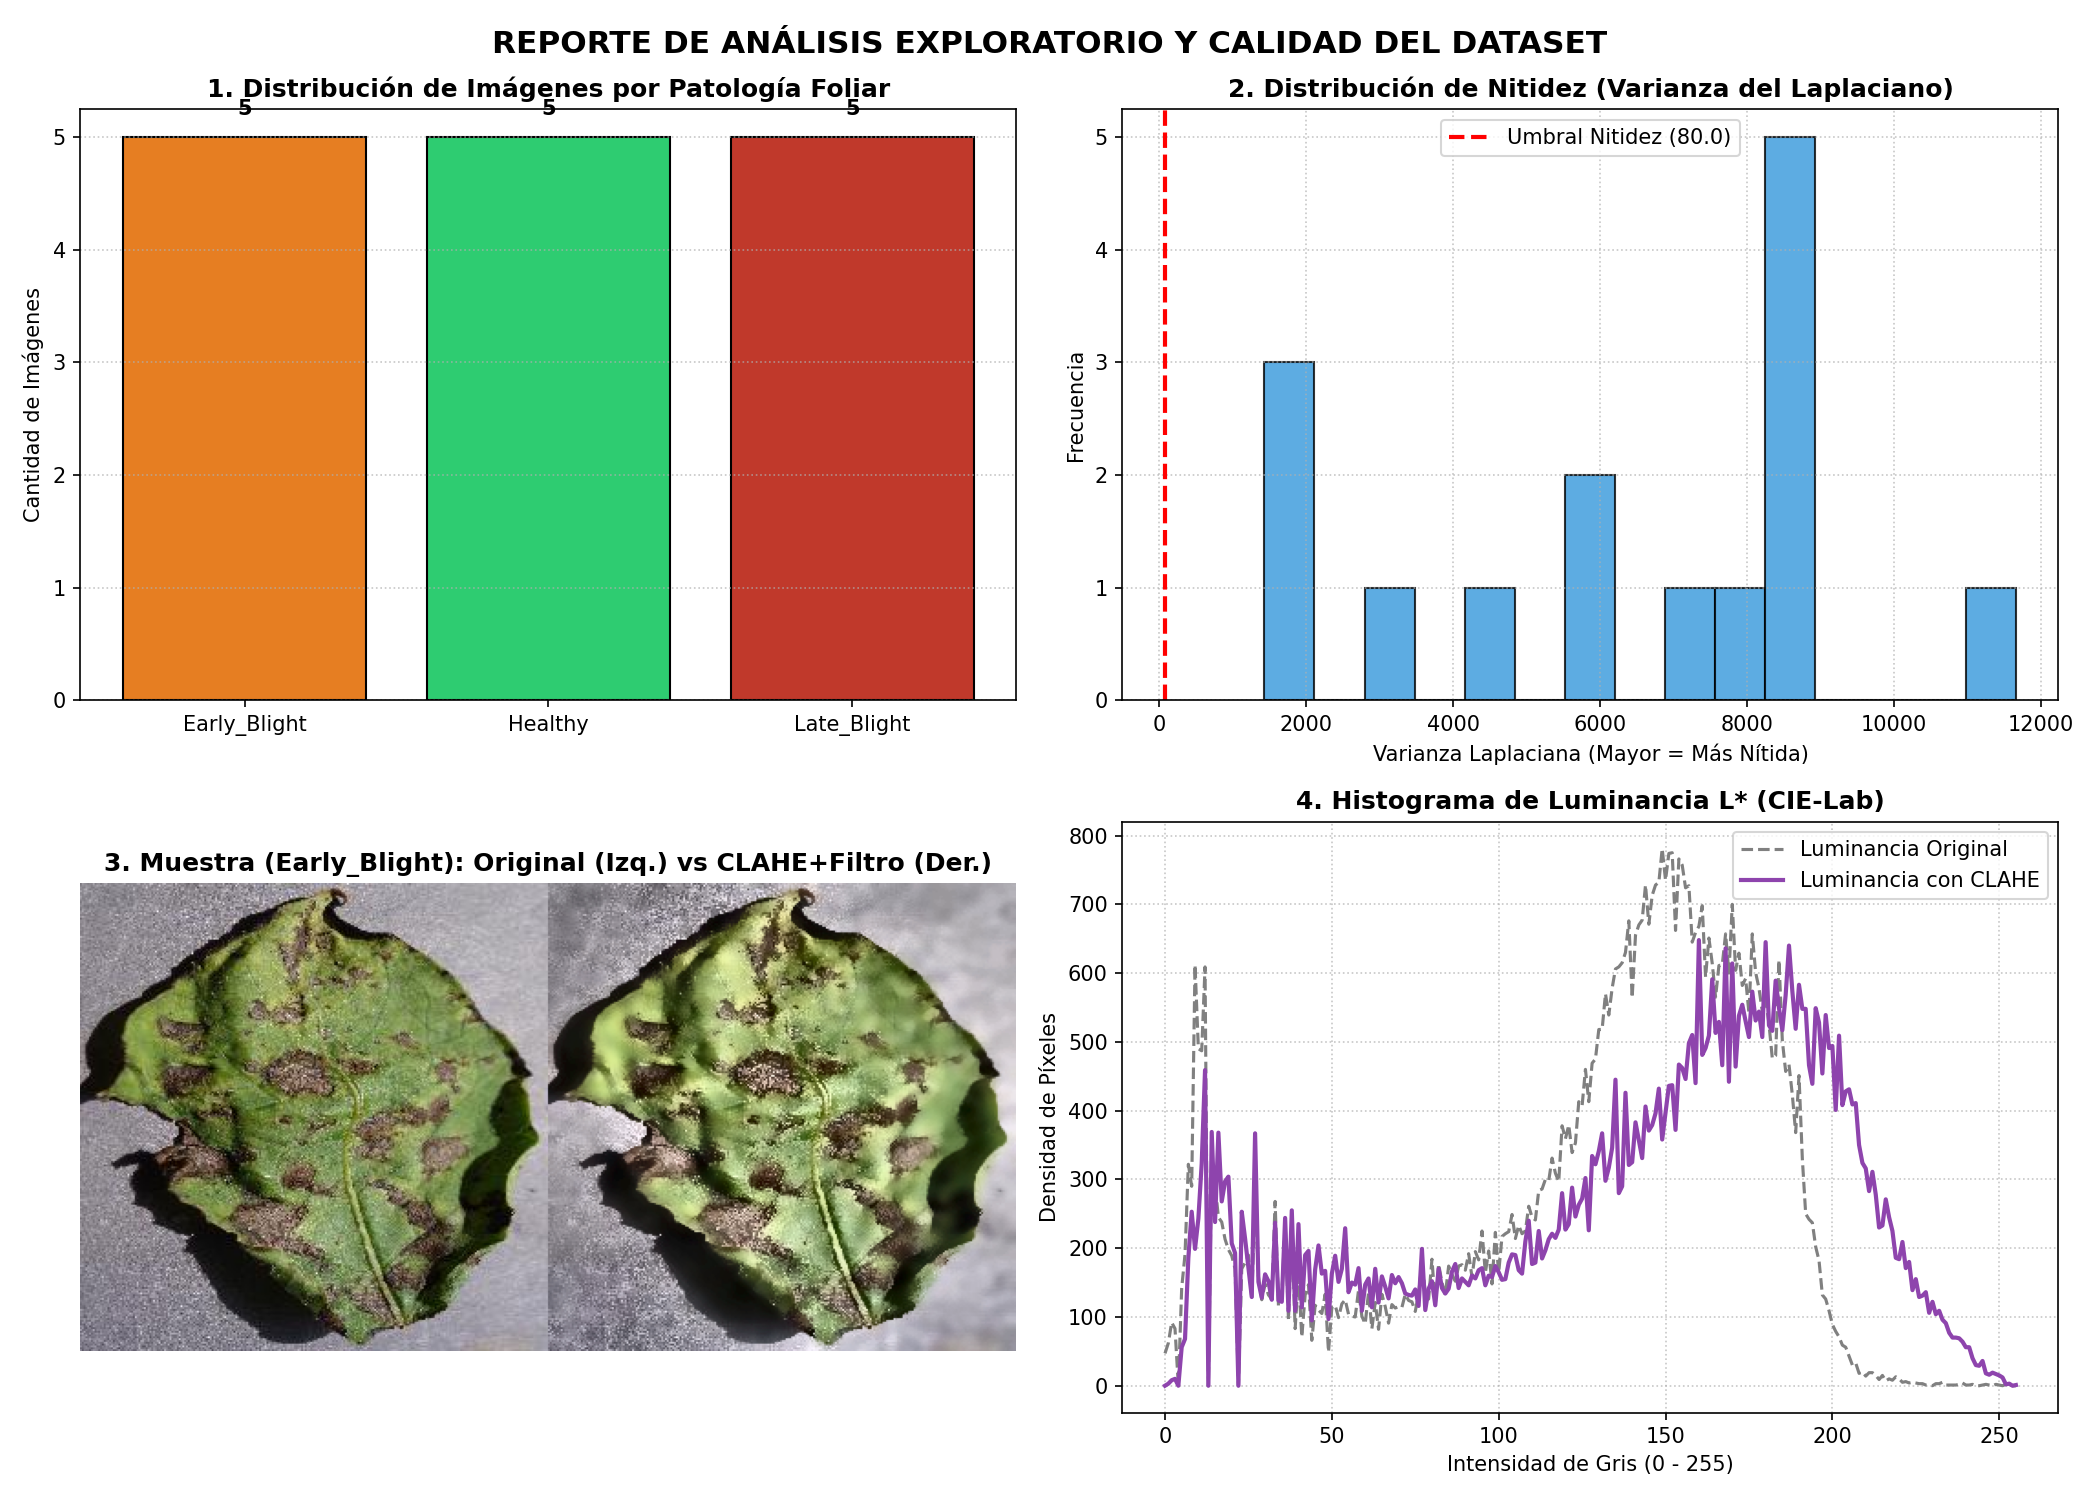
\includegraphics[width=0.92\textwidth]{eda_report.png}
    \caption{Panel integral de Análisis Exploratorio de Datos (EDA) del dataset foliar.}
    \label{fig:eda}
\end{figure}

% =========================================================================
% 5. GUÍA METODOLÓGICA PARA LA SUSTENTACIÓN ORAL
% =========================================================================
\section{Defensa Metodológica y Preguntas Clave de Sustentación}

Durante la evaluación de la entrega, el equipo preparó la fundamentación teórica para las interrogantes típicas formuladas por la cátedra:

\begin{enumerate}
    \item \textbf{¿Por qué no emplear una ecualización de histograma estándar global?} \\
    \textit{Fundamento:} La ecualización global asume una distribución uniforme acumulada en toda la escena. En imágenes foliares a cielo abierto, satura las áreas sobreexpuestas del fondo e incrementa severamente el ruido en regiones homogéneas. CLAHE opera localmente por teselas limitando la ganancia de gradiente, preservando los detalles sutiles de la hoja.
    
    \item \textbf{¿Por qué se transformó al espacio CIE-Lab en vez de operar directamente en RGB?} \\
    \textit{Fundamento:} El espacio RGB posee alta correlación cruzada entre canales; modificar intensidades en RGB altera el matiz biológico de la clorofila. CIE-Lab desacopla ortogonalmente la información acromática ($L^*$) de los componentes cromáticos ($a^*, b^*$), permitiendo realzar lesiones necróticas sin falsear los colores de la planta.
    
    \item \textbf{¿Por qué no aumentar el conjunto de prueba y validación?} \\
    \textit{Fundamento:} Las particiones de validación y test deben representar fielmente la distribución empírica no manipulada del entorno real. Aumentar sintéticamente estos conjuntos distorsionaría las métricas de generalización y produciría un sobreajuste inadvertido (\textit{data leakage}).
\end{enumerate}

% =========================================================================
% 6. CONCLUSIONES Y TRABAJO FUTURO
% =========================================================================
\section{Conclusiones y Trabajo Futuro}

\begin{itemize}
    \item Se consolidó un pipeline de preprocesamiento modular, reproducible y matemáticamente sustentado, que estandariza las muestras foliares a $256 \times 256$ píxeles conservando su relación de aspecto biológica.
    \item La combinación de filtrado bilateral y CLAHE en espacio CIE-Lab demostró una notable capacidad para amplificar micro-lesiones patológicas minimizando artefactos de captura.
    \item El particionado estratificado y el aumento selectivo en entrenamiento previenen fugas de información y garantizan una base de datos balanceada y de alta fidelidad.
    \item \textbf{Segunda Entrega:} Con la base preprocesada, se procederá a la extracción de descriptores morfológicos y de textura (matrices de coocurrencia GLCM, momentos invariantes de Hu) y al entrenamiento de arquitecturas de clasificación convolucionales (ResNet / MobileNet) orientadas a despliegue móvil.
\end{itemize}

% =========================================================================
% 7. REFERENCIAS BIBLIOGRÁFICAS
% =========================================================================
\section*{Referencias Bibliográficas}
\begin{enumerate}
    \item Gonzalez, R. C., \& Woods, R. E. (2018). \textit{Digital Image Processing} (4th ed.). Pearson.
    \item Szeliski, R. (2022). \textit{Computer Vision: Algorithms and Applications} (2nd ed.). Springer.
    \item Tomasi, C., \& Manduchi, R. (1998). \textit{Bilateral filtering for gray and color images}. In Sixth International Conference on Computer Vision (ICCV), IEEE, pp. 839--846.
    \item Pizer, S. M., et al. (1987). \textit{Adaptive histogram equalization and its variations}. Computer Vision, Graphics, and Image Processing, 39(3), 355--368.
    \item Mohanty, S. P., Hughes, D. P., \& Salathé, M. (2016). \textit{Using deep learning for image-based plant disease detection}. Frontiers in Plant Science, 7, 1419.
\end{enumerate}

\end{document}
